%! suppress = Makeatletter
%! suppress = Makeatletter
\documentclass[11pt]{report}

\usepackage[T1]{fontenc}
\usepackage[utf8]{inputenc}
\usepackage{graphicx}
\usepackage{amsmath,amssymb,amsfonts}
\usepackage{polski}
\usepackage[raggedright]{titlesec}
\usepackage{indentfirst}
\usepackage{listings}
\usepackage{hyperref}
\usepackage[backend=biber, bibencoding=utf8, style=ieee, dashed=false, isbn=false, doi=false, sorting=anyvt]{biblatex}
\usepackage{caption}
\captionsetup{%
justification=raggedright,
labelfont=bf,
singlelinecheck=off
}

%\addbibresource{library.bib}
\addbibresource{NEW.bib}

\pagestyle{headings}

\renewcommand{\chaptername}{Rozdział}
\renewcommand{\contentsname}{Spis treści}
\renewcommand{\figurename}{Rys.}
\renewcommand{\tablename}{Tab.}
\renewcommand{\listfigurename}{Spis rysunków}
\renewcommand{\listtablename}{Spis tabel}
\renewcommand{\bibname}{Bibliografia}

\makeatletter
\renewcommand{\l@section}{\@dottedtocline{1}{1.5em}{2.6em}}
\renewcommand{\l@subsection}{\@dottedtocline{2}{4.0em}{3.6em}}
\renewcommand{\l@subsubsection}{\@dottedtocline{3}{7.4em}{4.5em}}
\makeatother

\begin{document}
    \begin{titlepage}
        \centering
        
\includegraphics[width=\linewidth]{fig/AGH.jpg}
        \center{\scshape WYDZIAŁ INFORMATYKI, ELEKTRONIKI\\ i~TELEKOMUNIKACJI}
        \vspace{0.03\textheight}
        \center{\textbf PRACA DYPLOMOWA MAGISTERSKA}
        \vspace{0.03\textheight}
        \center{\LARGE\bfseries Agentowe środowisko do sterowania procesem identyfikacji i analizy wzorców czasowych w~notkach o zdarzeniach politycznych}
        \center{Multi-agent environment for management of the process of identifying and~analyzing time patterns in news about political events}
        \vspace{0.12\textheight}
        \begin{tabbing}
            \hspace{0.3\textwidth}\=\\
            Autor: \>Michał Patyk\\
            Kierunek studiów:\> Informatyka\\
            Opiekun pracy:\> dr hab.
            inż.
            Jarosław Koźlak
        \end{tabbing}
        \vspace{0.04\textheight}
        \center{Kraków 2021}
%        TODO: remove next line
        \center{wersja 0.1.5}
    \end{titlepage}

    \tableofcontents


    \chapter{Wstęp}\label{ch:wstęp}


    \chapter{Przegląd dziedziny}\label{ch:przegląd-dziedziny}
    W tym rozdziale w części~\ref{subsec:gdelt} opisany został zbiór GDELT\@.


    \section{Wzorce}

    \subsection{Ogólne}

    \subsubsection{Wzorce w sieciach społecznościowych}
    W pracy~\cite{10.1093/jigpal/jzaa042} autorzy identyfikują i kategoryzują wzorce opisujące interakcje między użytkownikami w sieciach społecznościowych.
    Uwaga została skupiona na wzorcach w których występują częste interakcje dwóch lub więcej użytkowników oraz na pozycji społecznej tych użytkowników w sieci.
    Zbiór danych został podzielony na N okien czasowych.
    Lista postów była eksportowana dla każdego okna, a na jej podstawie tworzono słownik.
    Przy pomocy słownika analizowano relacje miedzy użytkownikami.

    W pracy Odkrywanie ukrytych informacji w mediach społecznościowych~\cite{Skwara2019} autor bada częste lub nietypowe wzorce zachowań użytkowników mediów społecznościowych.
    Wzorce: wierny komentator, cięty komentator, dwaj komentatorzy, dwóch na jednego, komentator dwóch autorów, czujny komentator, prawo przechodniości.

    \subsection{GDELT}\label{subsec:gdelt}
    Celem pracy~\cite{Jarosz2020} identyfikacja wzorców w GDELT oraz opracowanie i ewaluacja algorytmów oraz metod analizy wzorców z tego zbioru\@.
    Badane wzorce zostały podzielone na statyczne oraz dynamiczne.
    Głównymi wyszczególnionymi elementami relacji sa powtarzalność oraz intensywność.
    Wzorce statyczne: sojusznik, nieprzyjaciel, symetria, asymetria, istotność, mocarstwo-klient.
    Wzorce dynamiczne: stabilna relacja, jedyna zmiana, pojedyncze zaburzenie, oscylacja, wzajemność, podobny ciąg dopasowań, zależność w czasie.
    Dodatkowe wzorce dynamiczne COVID-19: spadek nastrojów, nowa normalność, gratulacje, skupienie na walce.


    \section{Zastosowania}
    W pracy~\cite{Yan2012} autorzy proponują framework oparty na ważności dla charakteryzowania i wyodrębniania zmieniających sie wzorców w sieciach przedstawiających notatki prasowe.
    Zdefiniowano dwa wskaźniki istotności, aby scharakteryzować ewolucję i odkryć zmiany topologii o doniosłym znaczeniu.
    Cały proces znajdowania zachowań dynamicznych jest kierowany przez punktację istotności.

    \subsection{inne}\label{subsec:inne}
    Do analizy~\cite{Buckingham2020,Levin2018,Yuan2017}.


    \section{Systemy Agentowe}
    Według definicji z książki Grharda Weissa Systemy Wieloagentowe~\cite{55066420130101} agent to system komputerowy który jest umieszczony w pewnym środowisku i jest zdolny do autonomicznych akcji w tym środowisku w celu osiągnięcia wyznaczonych mu celów.
    Rysunek~\ref{fig:agent} przedstawia agenta w jego środowisku.
    \begin{figure}[!htp]
        \centering
        \includegraphics[width=\linewidth]{fig/agent_środowisko_weiss.png}
        \caption{Agent w swoim środowisku. (źródło: Multiagent Systems~\cite{55066420130101})}
        \label{fig:agent}
    \end{figure}
    Główną różnicą między agentami i obiektami jest stopień autonomiczności.
    Agenci nie wykonują nawzajem swoich metod ale raczej żądają wykonania czynności.
    Są zdolni reagowania, proaktywności i zachowań społecznych.
    Agent na podstawie swoich przekonań podejmuje najlepsze według niego decyzje.

    \subsection{Zalety Systemu Wieloagentowego}
    Główną zaletą wykorzystania systemu agentowego według Gerharda Weissa~\cite{55066420130101} jest możliwość samodzielnego decydowania przez system o tym co powinien zrobić w celu osiągnięcia celów mu wyznaczonych.
    Agenci którzy mogą działać w zmieniającym się, nieprzewidywalnym środowisku gdzie wykonywane akcje mogą się nie powieść nazywani są agentami inteligentnymi.
    Kolejna zaletą SA jest utrzymywanie równowagi między skupieniem na celu i reagowaniem na bodźce.
    Możliwość negocjacji i kooperacji.

    Obiekt nie jest zdolny do proaktywnego zachowania i nie jest w stanie samodzielnie decydować, co zrobić w określonej sytuacji.
    Autonomiczne komponenty oddelegowane do własnej kontroli mogą zostać wzbogacone o wyrafinowane umiejętności społeczne, to znaczy zdolność do podejmowania decyzji o zakresie i naturze ich interakcji w czasie wykonywania oraz inicjowania interakcji w sposób elastyczny (np. poprzez wyszukiwanie i negocjowanie świadczenia usług oraz dostarczania danych).

    \section{Metodologie rozwoju Systemu Agentowego}
    Dziedzina inżynierii oprogramowania zorientowanej na agentów zajmuje się opracowywaniem systemów opartych na agentach oraz sposobami wspierania ich rozwoju.
    W szczególności ma na celu dostarczenie metodologii projektowania systemów agentowych oraz narzędzi pomocniczych.

    \subsection{RIO}
    W pracy~\cite{S095741740200070220020101} autorzy proponują metodologię RIO (Roles, Interactions and Organizations) jako właściwe podejście przy analizie i projektowaniu systemów wieloagentowych.
    \begin{figure}[!ht]
        \centering
        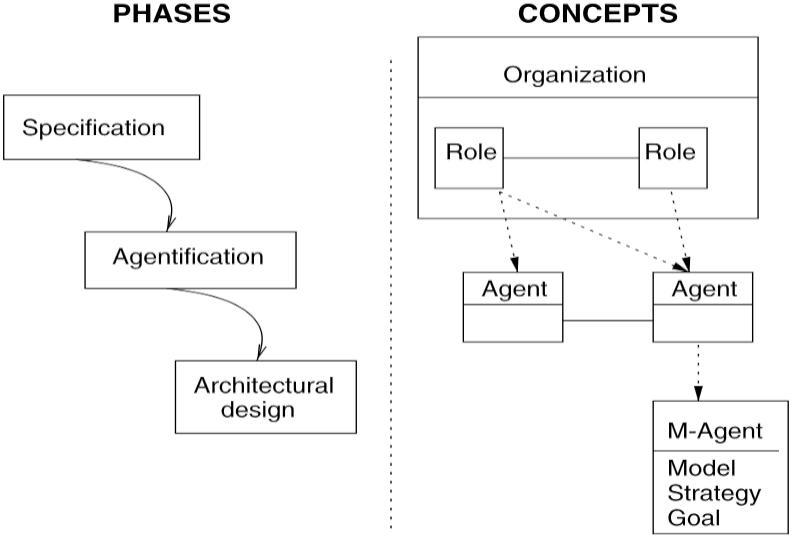
\includegraphics[width=\linewidth]{fig/RIO approach.png}
        \caption{Proces rozwoju w metodologii RIO. (źródło: A formal framework for multi-agent systems analysis and design \cite{S095741740200070220020101})}
        \label{fig:rio}
    \end{figure}
    System jest postrzegany jako organizacja która składa się ze zbioru wchodzących w interakcję ról.
    Role złożone powinny być dekomponowane na prostsze.
    Proces projektowania, przedstawiony na rysunku~\ref{fig:rio}, składa się z dwóch etapów: agentyfikacji i projektowania architektonicznego.
    Agentyfikacja to przypisanie roli do agentów.
    Na tym etapie nie robi się założeń co do architektury agentów.
    Dopiero etap projektowania architektonicznego kładzie naciska na wewnętrzną architekturę agenta.

    \subsection{GAIA}
    W pracy~\cite{Wooldridge2000a} autorzy opisują metodologię analizy i projektowania systemu agentowego Gaia
    Została ona założona na bazie widzenia systemu wieloagentowego jako organizacji obliczeniowej składającej się z wielu oddziałujących ze sobą ról.
    Proces analizy i projektowania, przedstawiony na rysunku~\ref{fig:gaia}, może być postrzegany jako przyrostowe budowanie coraz bardziej złożonych modeli systemu który ma być stworzony.
    \begin{figure}[!ht]
        \centering
        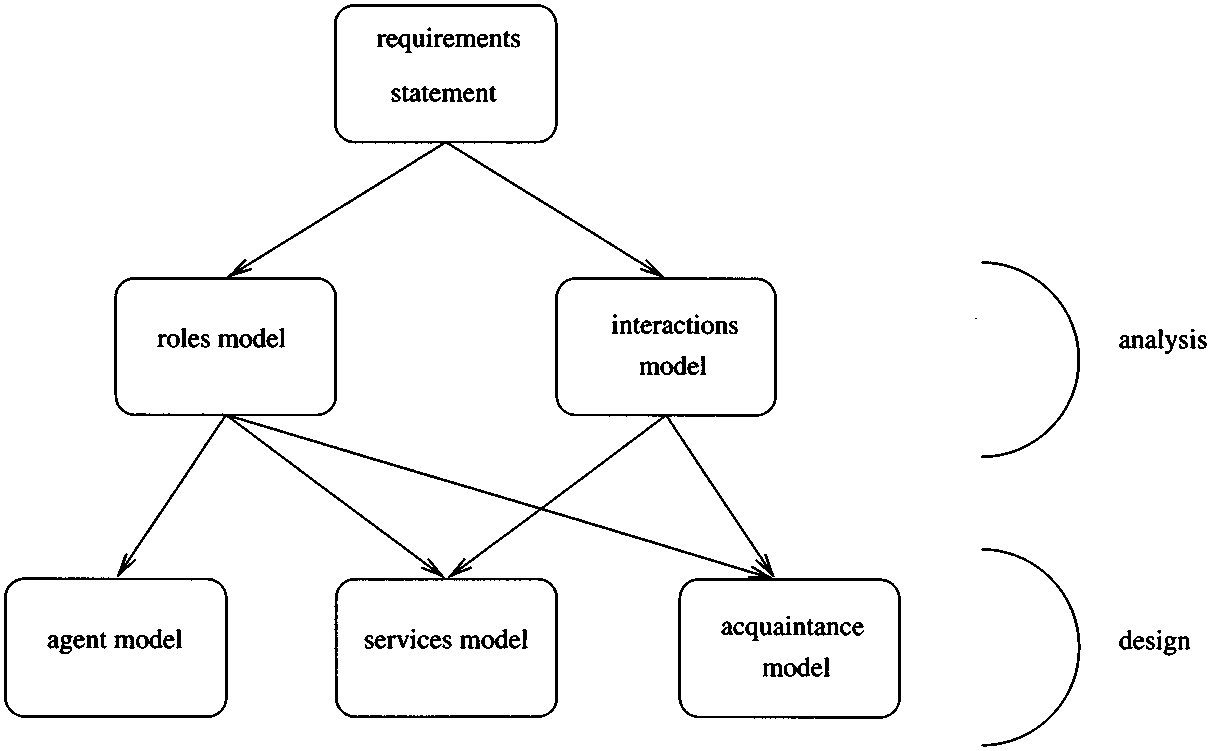
\includegraphics[width=\linewidth]{fig/gaia models.png}
        \caption{Zwiazek pomiędzy modelami Gaia. (źródło: The Gaia Methodology for Agent-Oriented Analysis and Design~\cite{Wooldridge2000a})}
        \label{fig:gaia}
    \end{figure}
    Celem etapu analizy jest rozwinięcie zrozumienia systemu i jego struktury.
    Podczas etapu projektowania Gaia skupia się na tym jak agenci mają kooperować aby zrealizować cele systemu oraz czego wymaga się od każdego agenta aby to osiągnąć.

    \subsection{GAIA v2}
    GAIA v2 jest oficjalnym rozszerzeniem metodologii.
    Role i protokoły są uzupełnione o środowisko, w którym działają agenci, specyfikujące jednostki i zasoby.
    Dodatkowe abstrakcje organizacyjne zostały przedstawione na rysunku~\ref{fig:gaia_v2}.
    \begin{figure}[!ht]
        \centering
        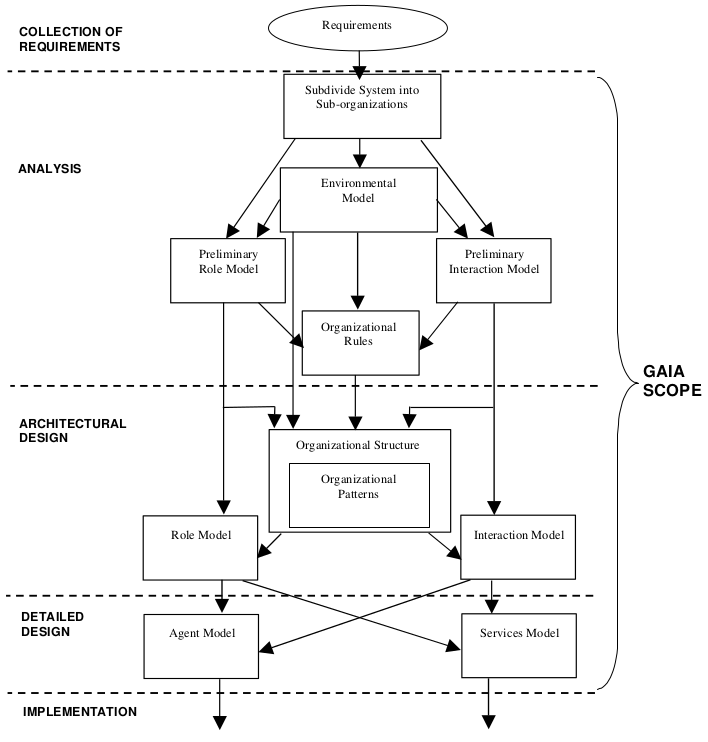
\includegraphics[width=\linewidth]{fig/gaia2 models.png}
        \caption{Modele i związki w GAIA v2. (źródło: Developing Multiagent Systems: The Gaia Methodology~\cite{Zambonelli2003})}
        \label{fig:gaia_v2}
    \end{figure}
    Reguły organizacyjne to ograniczenia które muszą być uwzględnione w globalnym zachowaniu organizacji.
    Struktura organizacyjna określa ogólną architekturę systemu.

    \subsection{ROADMAP}
    ROADMAP jest kolejnym rozszerzeniem metodologii GAIA.
    Faza analizy jest rozszerzona tak by pokryć również specyfikację.
    Wprowadzono dodatkowe modele opisujące środowisko oraz wiedze agentów.
    Rysunek~\ref{fig:roadmap} przedstawia strukturę modeli ROADMAP.
    \begin{figure}[!ht]
        \centering
        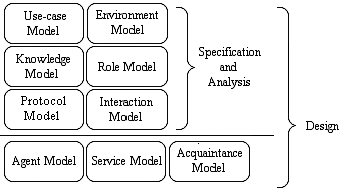
\includegraphics[width=\linewidth]{fig/roadmap models.png}
        \caption{Struktura modeli ROADMAP. (źródło: ROADMAP: Extending the Gaia methodology for complex open systems~\cite{Juan2002a})}
        \label{fig:roadmap}
    \end{figure}
    Hierarchia ról pełni podobną role do struktury i ról organizacyjnych w GAIA v2.
    Pozwala określić właściwe zachowanie agentów.

    \subsection{INGENIAS}
    W pracy~\cite{Pavon2003} autorzy przedstawiają metodologię rozwoju systemu wieloagentowego INGENIAS.
    Została ona zaprojektowana z myślą o budowie specyfikacji przyrostowo z zapewnieniem poprawności rozwoju.
    INGENIAS ulepsza oryginalne podejście z MESSAGE/UML poprzez dodanie nowego widoku oraz dostarczenie narzędzi do generowania kodu i dokumentacji systemu automatycznie ze specyfikacji.
    Generalnym podejściem INGENIAS do specyfikacji systemu wieloagentowego jest podział problemu na aspekty które tworzą różne widoki systemu.
    Każdy rodzaj widoku jest opisany z wykorzystaniem języka meta-modelującego.
    INGENIAS wyróżnia pięć metamodeli opisujących widoki, które muszą zostać wykorzystane przy opisie systemu:
    \begin{enumerate}
        \item Model agenta który opisuje pojedynczego agenta, jego zadania, cele, początkowy stan oraz role,
        \item Model interakcji który opisuje jakie interakcje mogą zajść między agentami,
        \item Model zadań i celów który opisuje relację między zadaniami i celami oraz ich strukturami,
        \item Model organizacji który opisuje jak komponenty systemu są ze sobą pogrupowane, jakie ograniczenia istnieją w interakcjach między agentami,
        \item Model środowiska który definiuje postrzeganie agentów jako elementów systemu oraz identyfikuje zasoby systemu.
    \end{enumerate}

    \subsection{Wnioski z przeglądu metodologii}
    \ldots


    W pracy z 2001 roku~\cite{Smirnov2002} autorzy przedstawiają technologię systemów wieloagentowych jako podstawę systemów Fuzji Wiedzy.
    Fuzje Wiedzy można zdefiniować jako integrację luźno powiązanych źródeł w połączone zasoby w celu uzupełnienia niedostatecznej wiedzy i uzyskania nowej.
    Korzystanie z inteligentnych agentów zwiększa wydajność i interoperacyjność systemu ponieważ agenci mogą działać w środowisku rozproszonym, niezależnie od użytkownika, i wykorzystywać
    ontologie do reprezentacji i wymiany wiedzy.


    \chapter{Koncepcja}\label{ch:koncepcja}
    Identyfikacja wzorców: opisujących państwa oraz relacje między państwami.
    Stworzenie reguł wspomagających odnajdywanie wzorców.

    Wejściem systemu jest zadanie konfiguracyjne.
    Zadanie konfiguracyjne uruchamia system który szuka wzorców.
    System zajmuje się:
    \begin{enumerate}
        \item rozdziałem zadań dla agentów,
        \item wyszukiwaniem wzorców,
        \item zbieraniem danych,
        \item analizą,
        \item generowaniem zestawień.
    \end{enumerate}

    Grupy agentów profilowane w celu automatycznego wyszukiwania wzorców czasowych.
    Zróżnicowanie agentów obejmuje:
    \begin{enumerate}
        \item progi,
        \item poziomy granulacji,
        \item wyszukiwanie korelacji,
        \item wyszukiwanie trendów,
        \item wykorzystanie dodatkowych źródeł informacji.
    \end{enumerate}

    Na wyjściu systemu otrzymujemy zagregowane dane.


    \section{Miary}
    Miary jakie zostaną wykorzystane do poszukiwania wzorców:
    \begin{enumerate}
        \item[•] liczby zdarzeń w~analizowanym okresie, w~których dany kraj jest aktorem 1 (dalej oznaczone jako \textit{Events}),
        \item[•] sumy liczby wzmianek (całkowitej liczby wzmianek o~tym wydarzeniu, we wszystkich dokumentach źródłowych podczas 15-minutowej aktualizacji, w~której zostało po raz pierwszy zauważone) w~analizowanym okresie, dla wydarzeń w~których dany kraj jest aktorem 1 (dalej oznaczone jako \textit{numMentions}),
        \item[•] stosunku liczby zdarzeń w~analizowanym okresie, w~których dany kraj jest aktorem 1, oznaczonych \textit{quad class} jako \textit{material conflict} do liczby zdarzeń w~analizowanym okresie, w~których dany kraj jest aktorem 1, oznaczonych \textit{quad class} jako \textit{material cooperation} (dalej oznaczone jako \textit{materialConfCoop}),
        \item[•] stosunku liczby zdarzeń w~analizowanym okresie, w~których dany kraj jest aktorem 1, oznaczonych \textit{quad class} jako \textit{verbal conflict} do liczby zdarzeń w~analizowanym okresie, w~których dany kraj jest aktorem 1, oznaczonych \textit{quad class} jako \textit{verbal cooperation} (dalej oznaczone jako \textit{verbalConfCoop}),
        \item[•] średniego, dla wszystkich zdarzeń w~analizowanym okresie, w~których dany kraj jest aktorem 1, średniego tonu (średni „ton” wszystkich dokumentów zawierających jedną lub więcej wzmianek o~tym wydarzeniu, podczas 15-minutowej aktualizacji, w~której zostało ono po raz pierwszy zauważone, waha się od -100 (skrajnie ujemny) do +100 (skrajnie dodatni)) (dalej oznaczone jako \textit{avgAvgTone}),
        \item[•] średniej, dla wszystkich zdarzeń w~analizowanym okresie, w~których dany kraj jest aktorem 1, miary Goldsteina (skala Goldsteina przypisuje wynik liczbowy od -10 do +10, wychwytując teoretyczny potencjalny wpływ, jaki rodzaj zdarzenia będzie miał na stabilność kraju) (dalej oznaczone jako \textit{avgGoldstein}),
        \item[•] liczby zdarzeń w~analizowanym okresie, w~których dany kraj jest aktorem 1, oznaczonych \textit{event root code} jako \textit{fight} Fight (dalej oznaczone jako \textit{fightCount}),
        \item[•] liczby zdarzeń w~analizowanym okresie, w~których dany kraj jest aktorem 1, oznaczonych \textit{event root code} jako \textit{Express intent to cooperate}  (dalej oznaczone jako \textit{expressCount}).
    \end{enumerate}


    \section{Wybór wzorców}

    \paragraph{GDELT}

    sojusznik
    nieprzyjaciel
    symetria
    asymetria
    mocarstwo-klient

    stabilna relacja
    pojedyncze zaburzenie
    oscylacja

    \paragraph{Bank Światowy}

    kraj rozwijający się
    bogaty kraj
    ubogi kraj


    \section{Role i Interakcje}

    \subsection{Role}
    Rola agenta określa, czego oczekuje się od niego zarówno w porozumieniu z innymi agentami, jak i w odniesieniu do całego systemu.
    Często rola agenta jest po prostu definiowana w kategoriach konkretnego zadania, które ma on wykonać w kontekście systemu.
    W metodologii GAIA rola jest definiowana przez cztery atrybuty~\cite{Wooldridge2000a}:
    \begin{enumerate}
        \item obowiązki,
        \item uprawnienia,
        \item aktywności,
        \item protokoły.
    \end{enumerate}
    Obowiązki determinują funkcjonalność i są podzielone na dwa typy:
    \begin{enumerate}
        \item właściwości żywotności - opisują te stany które agent musi wywołać, coś zostanie zrobione,
        \item właściwości bezpieczeństwa - sprawdzają po każdym wykonaniu czy stan jest akceptowalny.
    \end{enumerate}
    Uprawnienia to prawa związane z rolą.
    Identyfikują zasoby które sa dostępne dla danej roli w celu realizacji obowiązków.
    Działania to obliczenia związane z rolą, które mogą być przeprowadzone przez agenta bez interakcji z innymi.
    Protokoły definiują sposób w jaki role wchodzą w interakcję ze sobą.

    \begin{enumerate}
        \item Poszukiwacz wzorców
        \begin{enumerate}
            \item Poszukiwacz wzorców w danych GDELT
            \begin{enumerate}
                \item Poszukiwacz Wzorców Statycznych
                \begin{enumerate}
                    \item sojusznik
                    \item nieprzyjaciel
                    \item symetria
                    \item asymetria
                    \item mocarstwo-klient
                \end{enumerate}
                \item Poszukiwacz Wzorców Dynamicznych
                \begin{enumerate}
                    \item stabilna relacja
                    \item pojedyncze zaburzenie
                    \item oscylacja
                \end{enumerate}
                \item Poszukiwacz Wzorców Covid?
            \end{enumerate}
            \item Poszukiwacz wzorców w danych Banku Światowego
            \begin{enumerate}
                \item Poszukiwacz Wzorców Statycznych
                \begin{enumerate}
                    \item kraj rozwijający się
                    \item bogaty kraj
                    \item ubogi kraj
                \end{enumerate}
            \end{enumerate}
        \end{enumerate}
        \item Poszukiwacz Korelacji
        \item Poszukiwacz Trendów
        \item Generator Zestawień
    \end{enumerate}

    \subsection{Interakcje}
    W systemie zamkniętym wszyscy agenci są znani a priori i mają ze sobą współpracować, a zatem mogą sobie ufać podczas interakcji.
    W metodologii GAIA model interakcji składa się ze zbioru definicji protokołów.
    Protokół to wzorzec interakcji który został formalnie zdefiniowany i wyodrębniony.

    \begin{enumerate}
        \item Zgłoszenie znalezionej informacji przez agenta szukającego wzorców do agenta poszukującego korelacji i trendów.
        \item Przekazanie informacji do agenta generującego zestawienia.
    \end{enumerate}

    \begin{table}[ht!]
        \begin{tabular}{ll}
            Schemat roli:          & nazwa roli                                          \\ \hline
            Opis                   & krotki opis roli w języku polskim                   \\
            Protokoły i Aktywności & protokoły i aktywności w których rola bierze udział \\
            Uprawnienia            & prawa związane z rolą                               \\
            Obowiązki              &                                                     \\
            ~~żywotność            & obowiązki życiowe                                   \\
            ~~bezpieczeństwo       & odpowiedzialność za bezpieczeństwo                  \\
        \end{tabular}
        \caption{Schemat opisu roli agenta w metodologii GAIA. (źródło: Opracowanie własne)}
        \label{tab:schemat roli}
    \end{table}

    \begin{table}[ht!]
        \begin{tabular}{ll}
            Schemat roli:          & PoszukiwaczKorelacji                                           \\ \hline
            Opis                   & Ta rola obejmuje wyszukiwanie korelacji między krajami         \\
            & na podstawie danych pobranych od poszukiwaczy wzorców.         \\
            Protokoły i Aktywności & \textbf{sprawdzajWzorce, szukajKorelacji, poinformujGenerator} \\
            Uprawnienia            & \textbf{czyta dostarczone} \textit{PoszukiwaczWzorcow}         \\
            & ~~~~~~\textit{wzorzec}                                         \\
            & \textbf{zmienia} \textit{zestawienie}                          \\
            Obowiązki              &                                                                \\
            ~~żywotność            & \textbf{sprawdzajWzorce, szukajKorelacji, poinformujGenerator} \\
            ~~bezpieczeństwo       & -                                                              \\
        \end{tabular}
        \caption{Schemat roli Poszukiwacz Korelacji. (źródło: Opracowanie własne)}
        \label{tab:schemat roli poszukiwacz korelacji}
    \end{table}

    \begin{table}[ht!]
        \begin{tabular}{ll}
            Schemat roli:          & Generator Zestawień                                                          \\ \hline
            Opis                   & Ta rola obejmuje tworzenie zestawień na podstawie                            \\
            & danych zebranych przez poszukiwaczy korelacji i trendów.                     \\
            Protokoły i Aktywności & \textbf{sprawdzajZestawienia}                                                \\
            Uprawnienia            & \textbf{czyta dostarczone} \textit{PoszukiwaczKorelacji, PoszukiwaczTrendow} \\
            & ~~~~~~\textit{zestawienie}                                                   \\
            & \textbf{zmienia} \textit{zestawienie}                                        \\
            Obowiązki              &                                                                              \\
            ~~żywotność            & \textbf{sprawdzajZestawienia}                                                \\
            ~~bezpieczeństwo       & -                                                                            \\
        \end{tabular}
        \caption{Schemat roli Generator Zestawień. (źródło: Opracowanie własne)}
        \label{tab:schemat roli Generator Zestawień}
    \end{table}

    \begin{table}[ht!]
        \begin{tabular}{ll}
            Schemat roli:          & Poszukiwacz Wzorców                             \\ \hline
            Opis                   & Ta rola obejmuje wyszukiwanie wzorców           \\
            & pośród danych z wykorzystaniem zestawu miar.    \\
            & Wzorce dzielą się na dwie kategorie: wewnętrzne \\
            & oraz między krajami.                            \\
            Protokoły i Aktywności & \textbf{SzukajWzorców}                          \\
            Uprawnienia            & \textbf{czyta} \textit{miary}                   \\
            & \textbf{zmienia} \textit{wzorzec}               \\
            Obowiązki              &                                                 \\
            ~~żywotność            & \textbf{SzukajWzorców}                          \\
            ~~bezpieczeństwo       & -                                               \\
        \end{tabular}
        \caption{Schemat roli Poszukiwacz Wzorców. (źródło: Opracowanie własne)}
        \label{tab:schemat roli Poszukiwacz Wzorców}
    \end{table}

    \subsection{Agenci}
    Zadanie konfiguracyjne będzie określało na jakich krajach będzie skupiona uwaga systemu.
    Dla każdego kraju powstanie agent mu odpowiadający który obliczy podstawowe miary.
    Agenci przyjmujący role poszukiwaczy wzorców będą współpracować z agentami - krajami.

    Na podstawie ogólnego schematu Poszukiwacz Wzorców zostaną wyspecyfikowani poszukiwacze wzorców lokalnych - wewnętrznych -
    i globalnych - między państwami.
    Analizowane będą wzorce statyczne i dynamiczne.

    Agent związany z danym krajem może wstępnie badać relacje z innymi krajami i w razie potrzeby powołać agenta badającego relacje między krajami.


    \section{Współdziałanie agentów}
    Na rysunku~\ref{fig:relacje} przedstawiony został schemat relacji ról agentów.
    \begin{figure}[!ht]
        \centering
        \includegraphics[width=\linewidth]{fig/relacja ról.png}
        \caption{Interakcje ról. (źródło: Opracowanie własne)}
        \label{fig:relacje}
    \end{figure}


    \section{Eksploracja}

    \paragraph{Symetria relacji między państwami}
    Siła powiązania, zaproponowana w artykule, obliczana jest jako stosunek liczby zdarzeń pomiędzy krajem A, a krajem B, do liczby wszystkich zdarzeń w których kraj A jest aktorem 1.
    Ponieważ siła powiązania nie jest znormalizowana przez liczbę zdarzeń dla kraju B, dlatego nie jest symetryczna.
    Odzwierciedla to jak ważny dla kraju A jest kraj B.
    W trakcie eksploracji możliwe są zmiany miary symetrii np.:
    \begin{enumerate}
        \item poprzez wymnażanie przez liczbę wzmianek,
        \item wybór zdarzeń ważniejszych,
        \item filtrowanie miarą goldsteina.
    \end{enumerate}

    Wykres~\ref{fig:POL-DEU-POL} przedstawia symetryczność siły połączenia Polski i~Niemiec w~czasie.
    \begin{figure}[!htp]
        \centering
        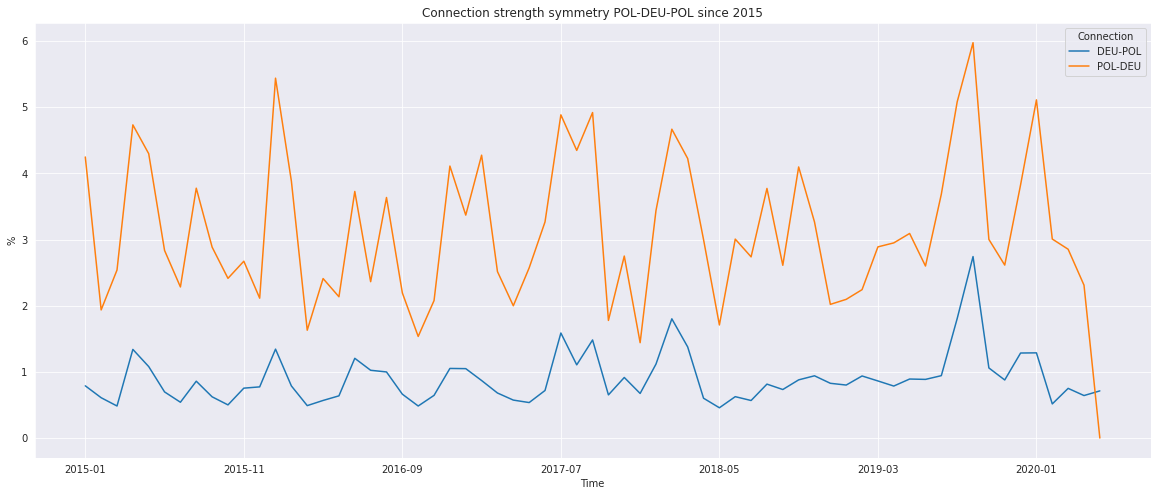
\includegraphics[width=\linewidth]{fig/POL-DEU-POL.png}
        \caption{Symetryczność siły połączenia Polski i~Niemiec w~czasie. (źródło: opracowanie własne)}
        \label{fig:POL-DEU-POL}
    \end{figure}


    Wykres~\ref{fig:POL-RUS-POL} przedstawia symetryczność siły połączenia Polski i~Rosji w~czasie.
    \begin{figure}[!htp]
        \centering
        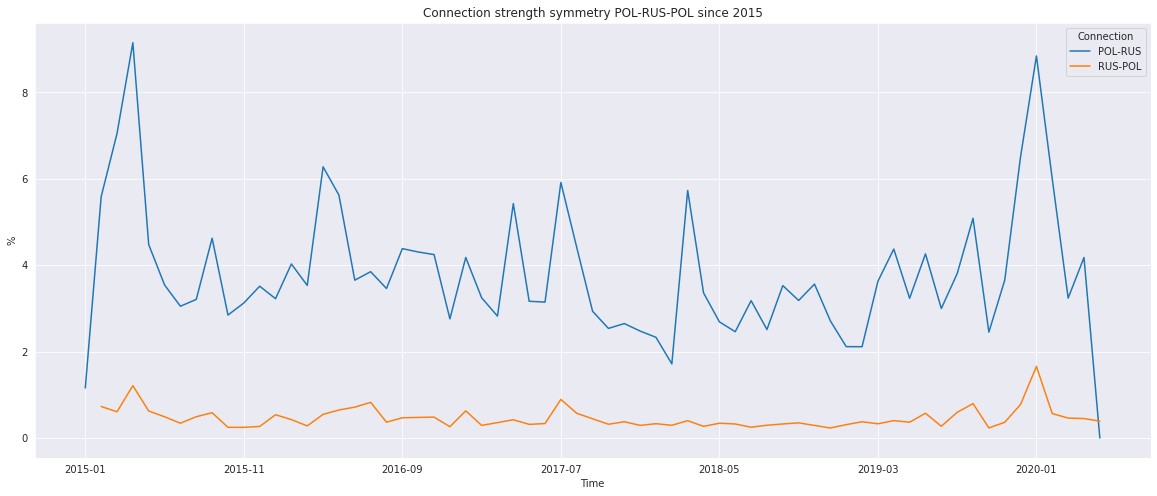
\includegraphics[width=\linewidth]{fig/POL-RUS-POL.png}
        \caption{Symetryczność siły połączenia Polski i~Rosji w~czasie. (źródło: opracowanie własne)}
        \label{fig:POL-RUS-POL}
    \end{figure}


    \chapter{Realizacja}\label{ch:realizacja}


    \section{Wybór systemu agentowego}

    W języku Python istnieje wiele bibliotek do analizy danych oraz uczenia maszynowego.
    Aby uniknąć potrzeby generowania powiązań z innymi językami platforma agentowa będzie również w Pythonie.
    Poniżej przeanalizowano zalety i wady kilku wybranych platform w tym języku.

    \subsection{Mesa}
    Mesa~\cite{Masad2015} to biblioteka do modelowania agentowego w Pythonie.
    Pozwala na szybkie stworzenie modelu agentowego przy wykorzystaniu wbudowanych komponentów.
    \href{https://github.com/projectmesa/mesa}{Project~Mesa~github}
    Ostatnie zmiany na githubie 28 listopada 2020 (stan na 11XII2020r.).

    \subsection{Python Agent DEvelopment framework}
    Framework PADE~\cite{Melo2019} umożliwia rozwój, wykonanie i zarządzanie wieloagentowymi systemami w rozproszonym środowisku.
    \href{https://github.com/grei-ufc/pade}{Smart~Grids~Research~Group~-~UFC~github}
    Ostatnie zmiany na githubie 22 maja 2020 (stan na 11XII2020r.).

    \subsection{Smart Python multi-Agent Development Environment}
    Platforma wieloagentowa SPADE jest oparta o XMPP\cite{Saint-Andre2007}.
    \href{https://github.com/javipalanca/spade}{javipalanca~github}
    Ostatnie zmiany na githubie 22 maja 2020 (stan na 11XII2020r.).


    \chapter{Ewaluacja}\label{ch:ewaluacja}


    \chapter{Podsumowanie}\label{ch:podsumowanie}

    \inputencoding{utf8}

    \newpage
    \addcontentsline{toc}{chapter}{Bibliografia}

%    TODO remove next line
    \nocite{*}
    \printbibliography[title={Bibliografia}]


\end{document}

